\documentclass{beamer}
\usepackage[utf8]{inputenc}
\usetheme{Berkeley}
\usecolortheme{seahorse}

\title{Sensores}
\subtitle{Os diferentes tipos de sensores e suas principais características.}

\AtBeginSection[]
{
	\begin{frame}
	\frametitle{Sumário}
	\tableofcontents[currentsection]
\end{frame}
}

\begin{document}

\frame{\titlepage}

\begin{frame}
	\frametitle{Sumário}
	\tableofcontents
\end{frame}

\section{Sentir}

\begin{frame}
	\frametitle{O que é sentir?!}
	sentir (verbo)
	\begin{itemize}
		\item perceber por qualquer dos sentidos.
		\item ter a impressão de algo.
	\end{itemize}
	{\scriptsize Fonte: Wiktionary.org (\url{https://pt.wiktionary.org/wiki/sentir})}\\
	\bigskip
	
	senciente (adjetivo)
	\begin{itemize}
		\item provido de sentimentos e sensações.
	\end{itemize}
	{\scriptsize Fonte: Wiktionary.org (\url{https://pt.wiktionary.org/wiki/senciente})}\\
\end{frame}

\begin{frame}
	\frametitle{Sistemas sensoriais}
	Aspectos do estímulo
	\begin{itemize}
		\item tipo (modalidade)
		\item intensidade
		\item localização
		\item duração
	\end{itemize}
	Objetivo de todo sistema sensorial:
	\begin{quote}
		``enviar as informações obtidas para o sistema nervoso central ou para alguma região que possa corretamente analisar e processar a informação.''
	\end{quote}
	{\scriptsize Fonte: Wikipedia (\url{https://pt.wikipedia.org/wiki/Sistema_sensorial})}
\end{frame}

\begin{frame}
	\frametitle{Sistemas sensoriais}
	Sentidos
	\begin{itemize}
		\item audição
		\item olfato
		\item paladar
		\item tato
		\item visão
	\end{itemize}
	Receptores sensoriais
	\begin{itemize}
		\item quimiorreceptores
		\item fotorreceptores
		\item mecanorreceptores
		\item termorreceptores
		\item nocirreceptores
	\end{itemize}
	{\scriptsize Fonte: Wikipedia (\url{https://pt.wikipedia.org/wiki/Sistema_sensorial})}
\end{frame}

\section{Tipos}

\begin{frame}
	\frametitle{Sensores e Transdutores}
	sensor (substantivo)
	\begin{itemize}
		\item dispositivo elétrico, eletrônico, mecânico ou biológico capaz de responder a estímulos de natureza física (temperatura, pressão, umidade, velocidade, aceleração, luminosidade e etc.); utilizado em sistemas de controle e monitoramento.
	\end{itemize}
	{\scriptsize Fonte: Wiktionary (\url{https://pt.wiktionary.org/wiki/sensor})}
	\bigskip
	
	transdutor (substantivo)
	\begin{itemize}
		\item um dispositivo que converte energia de uma forma em outra.
		\item (teoria da computação) uma máquina de estado que gera uma saída a partir de uma dada entrada.
	\end{itemize}
	{\scriptsize Fonte: Wiktionary (\url{https://en.wiktionary.org/wiki/transducer})}
\end{frame}

\begin{frame}
	\frametitle{Classificação de sensores}
		\begin{itemize}
			\item acústicos, de som, de vibração
			\item automotivos, para transportes
			\item químicos
			\item corrente elétrica, potencial elétrico, magnético, radio
			\item ambientais, de clima, umidade, vapor de água (\textit{moisture})
			\item fluxo, velocidade de fluidos
			\item giroscópio
			\item radiação ionizante, partículas subatômicas
			\item instrumentos de navegação
			\item ópticos, luz, imagem, fóton
			\item pressão
			\item força, densidade, nível
			\item térmicos, calor, temperatura
			\item proximidade, presença
			\item outros..
		\end{itemize}
		{\scriptsize Fonte: Wikipedia (\url{https://en.wikipedia.org/wiki/List_of_sensors})}
\end{frame}

\begin{frame}
	\frametitle{Um bom sensor}
	Espera-se de um bom sensor que ele siga as seguintes regras:
	\begin{itemize}
		\item ser sensível para a propriedade a ser medida;
		\item ser insensível para qualquer outra propriedade  a ser encontrada em sua aplicação; e
		\item não influenciar a propriedade a ser medida.
	\end{itemize}
	{\scriptsize Fonte: WIkipedia (\url{https://en.wikipedia.org/wiki/Sensor})}
\end{frame}

\section{Características}

\begin{frame}
	\frametitle{Características dos sensores}
	\begin{itemize}
		\item Sensibilidade
		\item Faixa
		\item Precisão
		\item Resolução
		\item Exatidão
		\item Offset
		\item Linearidade
		\item Histerese
		\item Tempos de resposta
		\item Linearidade dinâmica
	\end{itemize}
	{\scriptsize Fonte: J.J. Carr, Sensors and Circuits, Prentice Hall, 1993.}
\end{frame}

\begin{frame}
	\frametitle{Sensibilidade}
	A sensibilidade do sensor é definida como:
	 \begin{itemize}
	 	\item a inclinação da curva característica de saída ou, de forma mais geral, a mínima entrada do parâmetro físico que cria uma variação detectável na saída;
	 	\item a variação do parâmetro de entrada necessária para produzir uma variação padronizada na saída;
	 	\item uma variação na tensão de saída para uma dada variação no parâmetro de entrada.
	 \end{itemize}	
 	 Observação: O erro de sensibilidade é um deslocamento com relação à inclinação ideal da curva característica.
	{\scriptsize Fonte: J.J. Carr, Sensors and Circuits, Prentice Hall, 1993.}
\end{frame}

\begin{frame}
	\frametitle{Sensibilidade}
	\begin{figure}
		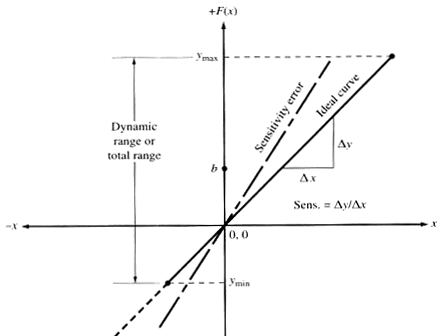
\includegraphics[width=0.9\textwidth]{sensibilidade}
	\end{figure}
	{\scriptsize Fonte: J.J. Carr, Sensors and Circuits, Prentice Hall, 1993.}
\end{frame}

\begin{frame}
	\frametitle{Faixa}
	A faixa do sensor segue as seguintes descrições:
	\begin{itemize}
		\item a faixa é determinada pelos valores mínimo e máximo do parâmetro em questão que podem ser medidos.
		\item não é necessário que as faixas positiva e negativa tenham a mesma extensão.
		\item faixa dinâmica é a faixa total do sensor entre o valor mínimo e o valor máximo.
	\end{itemize}
	{\scriptsize Fonte: J.J. Carr, Sensors and Circuits, Prentice Hall, 1993.}
\end{frame}

\begin{frame}
	\frametitle{Precisão}
	Algumas definições:
	\begin{itemize}
		\item  Refere-se ao grau de reproducibilidade de uma medição. Em outras palavras, medindo exatamente o mesmo valor várias vezes, um sensor ideal colocaria na saída exatamente o mesmo valor todas as vezes.
		\item Este conceito é normalmente interpretado como sendo a diferença que existe entre o valor medido e o valor real, normalmente expresso como uma porcentagem.
	\end{itemize}
	Questão: qual é a diferença entre precisão e acurácia?!\\
	\bigskip
	{\scriptsize Fonte: J.J. Carr, Sensors and Circuits, Prentice Hall, 1993; Instituto NCB (\url{http://www.newtoncbraga.com.br/index.php/eletronica/52-artigos-diversos/4888-art645})} 
\end{frame}

\begin{frame}
	\frametitle{Precisão}
	\begin{figure}
		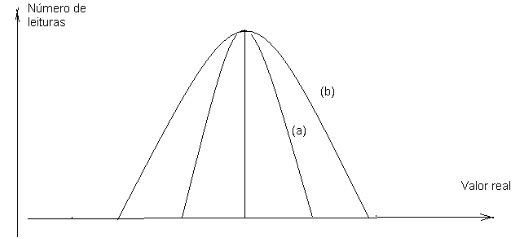
\includegraphics[width=0.9\textwidth]{precisao}
		\caption{Curvas de distribuição de uma medida para sensores (a) mais preciso e (b) menos preciso.}
	\end{figure}
	{\scriptsize Fonte: Instituto NCB (\url{http://www.newtoncbraga.com.br/index.php/eletronica/52-artigos-diversos/4888-art645})}
\end{frame}

\begin{frame}
	\frametitle{Resolução}
	A resolução de um sensor pode ser definida como:
	\begin{itemize}
		\item a menor variação incremental detectável do parâmetro de entrada que pode ser detectada no sinal de saída.
	\end{itemize}
	
	{\scriptsize Fonte: J.J. Carr, Sensors and Circuits, Prentice Hall, 1993.}
\end{frame}

\begin{frame}
	\frametitle{Exatidão}
	A exatidão do sensor pode ser definida como:
	\begin{itemize}
		\item a máxima diferença entre o valor real (medido por um padrão primário ou bom padrão secundário) e o valor indicado na saída do sensor.
	\end{itemize}
	{\scriptsize Fonte: J.J. Carr, Sensors and Circuits, Prentice Hall, 1993.}
\end{frame}

\begin{frame}
		\frametitle{Offset}
		O erro de offset de um transdutor é definido como:
		\begin{itemize}
			\item um valor de saída existente quando deveria ser zero
			\item a diferença entre o valor de saída real e o valor de saída especificado sob um determinado conjunto de condições.
		\end{itemize}  	
		{\scriptsize Fonte: J.J. Carr, Sensors and Circuits, Prentice Hall, 1993.}
\end{frame}

\begin{frame}
	\frametitle{Offset}
	\begin{figure}
		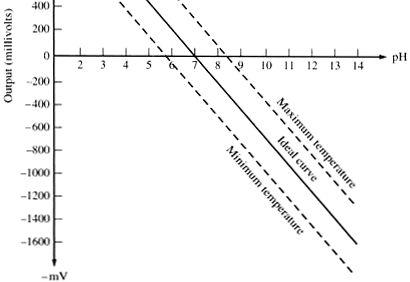
\includegraphics[width=0.8\textwidth]{offset}
		\caption{Curva característica de eletrodo de pH, mostrando a sensibilidade à temperatura.}
	\end{figure}  	
	{\scriptsize Fonte: J.J. Carr, Sensors and Circuits, Prentice Hall, 1993.}
\end{frame}

\begin{frame}
	\frametitle{Linearidade}
	A linearidade do transdutor é uma expressão do quanto a curva real medida de um sensor se afasta da curva ideal. 
	\begin{figure}
		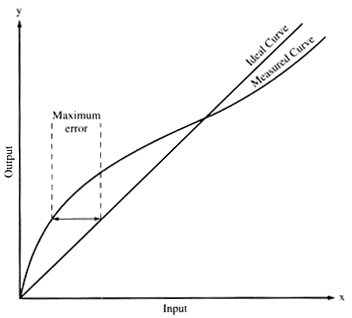
\includegraphics[width=0.5\textwidth]{linearidade}
		\caption{Curva ideal em comparação com a medida, mostrando erro de linearidade.}
	\end{figure} 
	{\scriptsize Fonte: J.J. Carr, Sensors and Circuits, Prentice Hall, 1993.}
\end{frame}


\begin{frame}
	\frametitle{Histerese}
	Um transdutor deve ser capaz de seguir as variações do parâmetro de entrada independentemente da direção na qual ocorre essa variação; a histerese é a medida dessa propriedade. 	
	\begin{figure}
		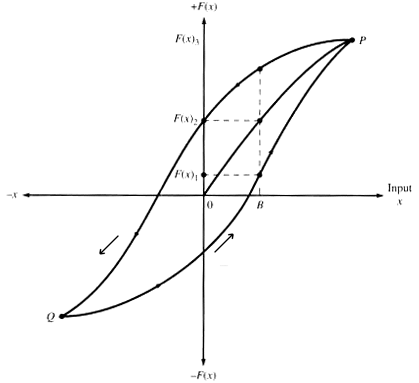
\includegraphics[width=0.45\textwidth]{histerese}
		\caption{Curva de histerese.}
	\end{figure} 
	{\scriptsize Fonte: J.J. Carr, Sensors and Circuits, Prentice Hall, 1993.}
\end{frame}

\begin{frame}
	\frametitle{Tempo de resposta}
	O tempo de resposta pode ser definido como:
	\begin{itemize}
		\item o tempo necessário para a saída de um sensor passar de um estado anterior a um valor estabilizado final dentro da banda de tolerância do novo valor correto.
	\end{itemize}
	{\scriptsize Fonte: J.J. Carr, Sensors and Circuits, Prentice Hall, 1993.}
\end{frame}

\begin{frame}
	\frametitle{Tempo de resposta}
	\begin{figure}
		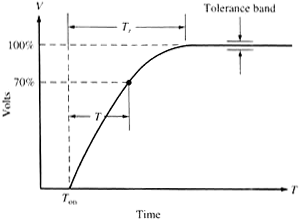
\includegraphics[width=0.7\textwidth]{tempoderespostasubida}
		\caption{Definição de tempo de subida.}
	\end{figure}  	
	{\scriptsize Fonte: J.J. Carr, Sensors and Circuits, Prentice Hall, 1993.}
\end{frame}

\begin{frame}
	\frametitle{Tempo de resposta}
	\begin{figure}
		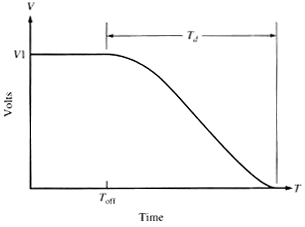
\includegraphics[width=0.7\textwidth]{tempoderepostadescida}
		\caption{Definição de tempo de descida.}
	\end{figure}  	
	{\scriptsize Fonte: J.J. Carr, Sensors and Circuits, Prentice Hall, 1993.}
\end{frame}

\begin{frame}
	\frametitle{Linearidade dinâmica}
	A linearidade dinâmica do sensor é a medida de sua capacidade de acompanhar mudanças rápidas do parâmetro de entrada.\\
	\bigskip
	Observação:	Características de \textbf{distorção de amplitude}, \textbf{distorção de fase} e \textbf{tempo de resposta} são importantes para a determinação da linearidade dinâmica.\\
	\bigskip
	{\scriptsize Fonte: J.J. Carr, Sensors and Circuits, Prentice Hall, 1993.}
\end{frame}

\begin{frame}
	\frametitle{Linearidade dinâmica}
	\begin{figure}
		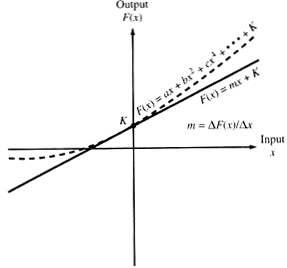
\includegraphics[width=0.6\textwidth]{linearidadedinamicaerroquadratico}
		\caption{Curva de saída e entrada do sinal, mostrando erro quadrático.}
	\end{figure}  	
	{\scriptsize Fonte: J.J. Carr, Sensors and Circuits, Prentice Hall, 1993.}
\end{frame}

\frame{\titlepage}

\end{document}
